\input{../../header.tex}

\usepackage[section]{placeins}

\usepackage{csquotes}

\usepackage{tikz}
\usetikzlibrary{chains}
\usetikzlibrary{shapes.geometric}

\tikzset{device/.style={
                rectangle,
                minimum size=6mm,
                draw=black
            },
            monitor/.style={
                rectangle,
                rounded corners=2mm,
                minimum size=6mm,
                draw=black
            },
        }

\usepackage{pgfplots}
\pgfplotsset{
    compat=1.5,
    width=0.8\linewidth,
    xticklabel style={/pgf/number format/use comma},
    yticklabel style={/pgf/number format/use comma},
}

\usepgfplotslibrary{external}
\tikzexternalize

\DeclareSIUnit{\skt}{SKT}

\usepackage{booktabs}

\hypersetup{
    pdftitle=
}

\subject{Praktikumsprotokoll}
\title{Compton-Effekt}
\subtitle{Versuch P526 -- Universität Bonn}
\author{
    Martin Ueding \\ \small{\href{mailto:mu@martin-ueding.de}{mu@martin-ueding.de}}
    \and
    Lino Lemmer \\
    \small{\href{mailto:l2@uni-bonn.de}{l2@uni-bonn.de}}
}

\date{\daterange{2014-04-24}{2014-04-25}}

% TODO Tutor Eintragen
%\publishers{Tutor: TODO}

\begin{document}

\maketitle

\begin{abstract}
\end{abstract}

\tableofcontents

\chapter{Theorie}

\begin{figure}[htbp]
    \centering
    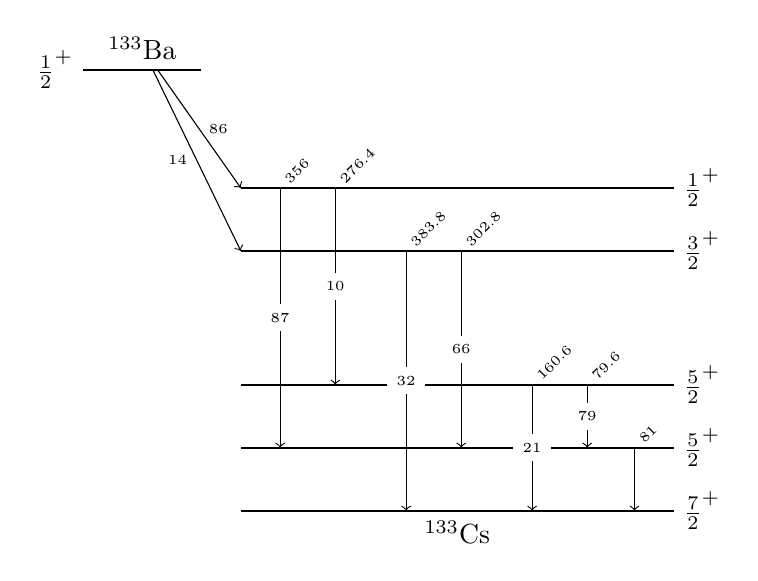
\begin{tikzpicture}
        \draw[thick]
        (-.5,5) node[left]{$\frac12^+$} -- node[above] (Ba) {${}^{133}$Ba} (1,5)
        (1.5,3.5) coordinate (EC1) -- (7,3.5) node[right] {$\frac12^+$}
        (1.5,2.7) coordinate (EC2) -- (7,2.7) node[right] {$\frac32^+$}
        (1.5,1.0)  -- (7,1.0) node[right] {$\frac52^+$}
        (1.5,0.2)  -- (7,0.2) node[right] {$\frac52^+$}
        (1.5,-0.6) -- node[below] {${}^{133}$Cs} (7,-0.6) node[right] {$\frac72^+$}
        ;
        \draw[->]
        (Ba) -- node[right]{\tiny{\SI{86}{\percent}}} (EC1)
        ;
        \draw[->]
        (Ba) -- node[left]{\tiny{\SI{14}{\percent}}} (EC2)
        ;
        % Linien
        \draw[->]
        (2,3.5) node[right, rotate=45]
        {\tiny{\SI{356}{\kilo\electronvolt}}} -- node[midway,
        fill=white] {\tiny{\SI{87}{\percent}}} (2,.2)
        ;
        \draw[->]
        (2.7,3.5) node[right, rotate=45]
        {\tiny{\SI{276.4}{\kilo\electronvolt}}} -- node[midway,
        fill=white] {\tiny{\SI{10}{\percent}}} (2.7,1.)
        ;
        \draw[->]
        (3.6,2.7) node[right, rotate=45]
        {\tiny{\SI{383.8}{\kilo\electronvolt}}} -- node[midway,
        fill=white] {\tiny{\SI{32}{\percent}}} (3.6,-.6)
        ;
        \draw[->]
        (4.3,2.7) node[right, rotate=45]
        {\tiny{\SI{302.8}{\kilo\electronvolt}}} -- node[midway,
        fill=white] {\tiny{\SI{66}{\percent}}} (4.3,.2)
        ;
        \draw[->]
        (5.2,1.0) node[right, rotate=45]
        {\tiny{\SI{160.6}{\kilo\electronvolt}}} -- node[midway,
        fill=white] {\tiny{\SI{21}{\percent}}} (5.2,-.6)
        ;
        \draw[->]
        (5.9,1.0) node[right, rotate=45]
        {\tiny{\SI{79.6}{\kilo\electronvolt}}} -- node[midway,
        fill=white] {\tiny{\SI{79}{\percent}}} (5.9,.2)
        ;
        \draw[->]
        (6.5,.2) node[right, rotate=45]
        {\tiny{\SI{81}{\kilo\electronvolt}}} -- (6.5,-.6)
        ;
    \end{tikzpicture}
    \caption{%
        Zerfallsschema von ${}^{133}$Ba. Übernommen aus \parencite{Ueding/525}.
    }
    \label{fig:Ba-Zerfall}
\end{figure}


\IfFileExists{\bibliographyfile}{
    \printbibliography
}{}

\end{document}

% vim: spell spelllang=de tw=79
